\chapter{Exploration 1: creating a command-line tutorial in XIMPEL}
\label{chap:exploration1}
Looking at the structure of many MOOCs, it could be observed that they all have a simple video playlist and then follow up with some multiple choice questions or a coding assignment within an online code editor. Is it not possible to recreate a command-line tutorial with XIMPEL? Because if it is, then it will be a lot quicker to create such an application compared to creating it from scratch!

On a related matter, with the implementation of a command-line tutorial, XIMPEL could compete with computer science courses on Coursera. It could not compete on design but on pragmaticism, not on flexibility but on programming simplicity, not on comprehensiveness but on development speed. With this extension, XIMPEL occupies a unique niche of hypermedia and education.

By recreating a command-line tutorial in XIMPEL I stumbled upon a question. A command-line interface is not a form of media. A command-line interface is an application. So by recreating this in XIMPEL I am mixing a computer application with hypermedia. What does this mean? Am I now leaving hypermedia? Are we mixing hypermedia elements with a computer application? Could XIMPEL still be considered a hypermedia framework? Should XIMPEL be a hypermedia framework in the first place? 

The questions that I will formally focus on in this exploration are: how would XIMPEL need to be extended in order to create a command-line tutorial? And what are the implications of mixing a hypermedia application with another (non hypermedia) application with regards to hypermedia as a field?

\section{Extending XIMPEL to create a command-line tutorial}
Did you know that the XIMPEL is an acronym for eXtensible Interactive Media Player for Entertainment and Learning? Neither did I at one point. The extensibility of this media player will be demonstrated here. Together with the core changes I made in the framework, it is even more extensible!

So is it possible to recreate a command-line tutorial with XIMPEL? The answer is yes. Our research question has been answered. I suppose we are done.

Which command-line tutorial are we recreating you might ask? From CodeCademy\footnote{\hyperlink{https://www.codecademy.com}{https://www.codecademy.com}} of course! It is one of the leading organizations for online programming education. To give a feel for how CodeCademy looks like I recommend you to try the command-line tutorial yourself. For readers who are reading this on paper, figure \ref{fig:codecademy} will show a screenshot from a part of the command-line tutorial.

\begin{figure}
    \centering
    \includegraphics[width=1.35\textwidth, center]{codecademy_example.png} % quotation marks make sure file name does not display
    \caption{A lesson in the Codecademy command-line tutorial. This lesson shows how to use the print working directory command.}
    \label{fig:codecademy}
\end{figure}

When I first started recreating this command-line tutorial I realized two things. (1) It would be interesting to see how such a tutorial would be with video besides it instead of text and (2) I did not have time to recreate the whole tutorial so by using my artistic freedom I recreated the first two lessons which are about how to use the `pwd` and the `ls` command. By doing this the framework is going towards online education. Media itself is in most cases already a form of education, but by creating a command-line tutorial the XIMPEL framework moves more towards the interactive part of education. 

% \section{Requirements command-line tutorial}
The command-line tutorial requires two things. XIMPEL needs to be extended in order to play multiple media types. It could be possible to create a media type that plays video and has a terminal emulator which is too tightly coupled. This gave rise to exploration 2. The other requirement is that XIMPEL needs to be able to have a terminal of some sort. In this exploration I will focus on how I created a terminal application within XIMPEL.

\section{Architecture of the command-line media type}
In order to create a proof of concept I started looking and reverse engineering on how other command-line web applications were created. I took a look at: R-fiddle and CodeCademy. I also took a look at JSfiddle since I entertained the idea of executing JavaScript as a code tutorial. I quickly stopped entertaining that idea when I realized I had to use the `eval` function and would create a whole host of additional security hazards to XIMPEL. 

R-fiddle has the following architecture: it has a client, a server and it communicates via websockets (seen via Chrome Developer Tools). It spins up a virtualized container such as docker or vagrant in order to minimize security risks such as a shell with too much privileges on a file system that has sensitive information. By using virtualized containers for each new client, there is no file system with sensitive information and the shell does not have too many privileges \cite{r-fiddle}.

Codecademy sends an authentication token to a server along with other data via an xhr-request (in JavaScript parlance: they use AJAX) and send other relevant data with it in order to manage at what course the user is and if the user is logged in. The server answers back in JSON. Also Codecademy uses websockets to communicate with a terminal application (see figure \ref{fig:codecademy_websockets}). Presumably, they use some form of sandboxing.

The common architecture in common with both websites are: client, server, websockets as communication and presumably sandboxing. So the first step I created was creating a command-line tutorial in HTML/JS/CSS. Once that was completed I realized I needed to implement the client-side facing part of the terminal as a XIMPEL media type. Moreover, that media type needs to connect via websockets to a server. 

\begin{figure}
\centering
\includegraphics[width=1.35\textwidth, center]{codecademy_websockets.png} % quotation marks make sure file name does not display
\caption{Evidence that CodeCademy uses websockets to communicate with a terminal on some server. The blue circles shows data that is sent from the client to the server. The red circles shows data that is sent from the server to the client.}
\label{fig:codecademy_websockets}
\end{figure}

The current implementation has its server-side part implemented in NodeJS with the web server micro framework ExpressJS, which currently receives input data from the XIMPEL terminal media type via websockets. It furthermore spawns a bash shell and sends the data back to the terminal media type. Once it is there, the output of the bash shell will be displayed in the XIMPEL presentation. It has to be stated that this implementation is a proof of concept as it is not secure since the bash shell is not sandboxed with Vagrant or Docker, for example. Figure \ref{images:terminal_architecture} illustrates the client-server communication.

\begin{figure}
\centering
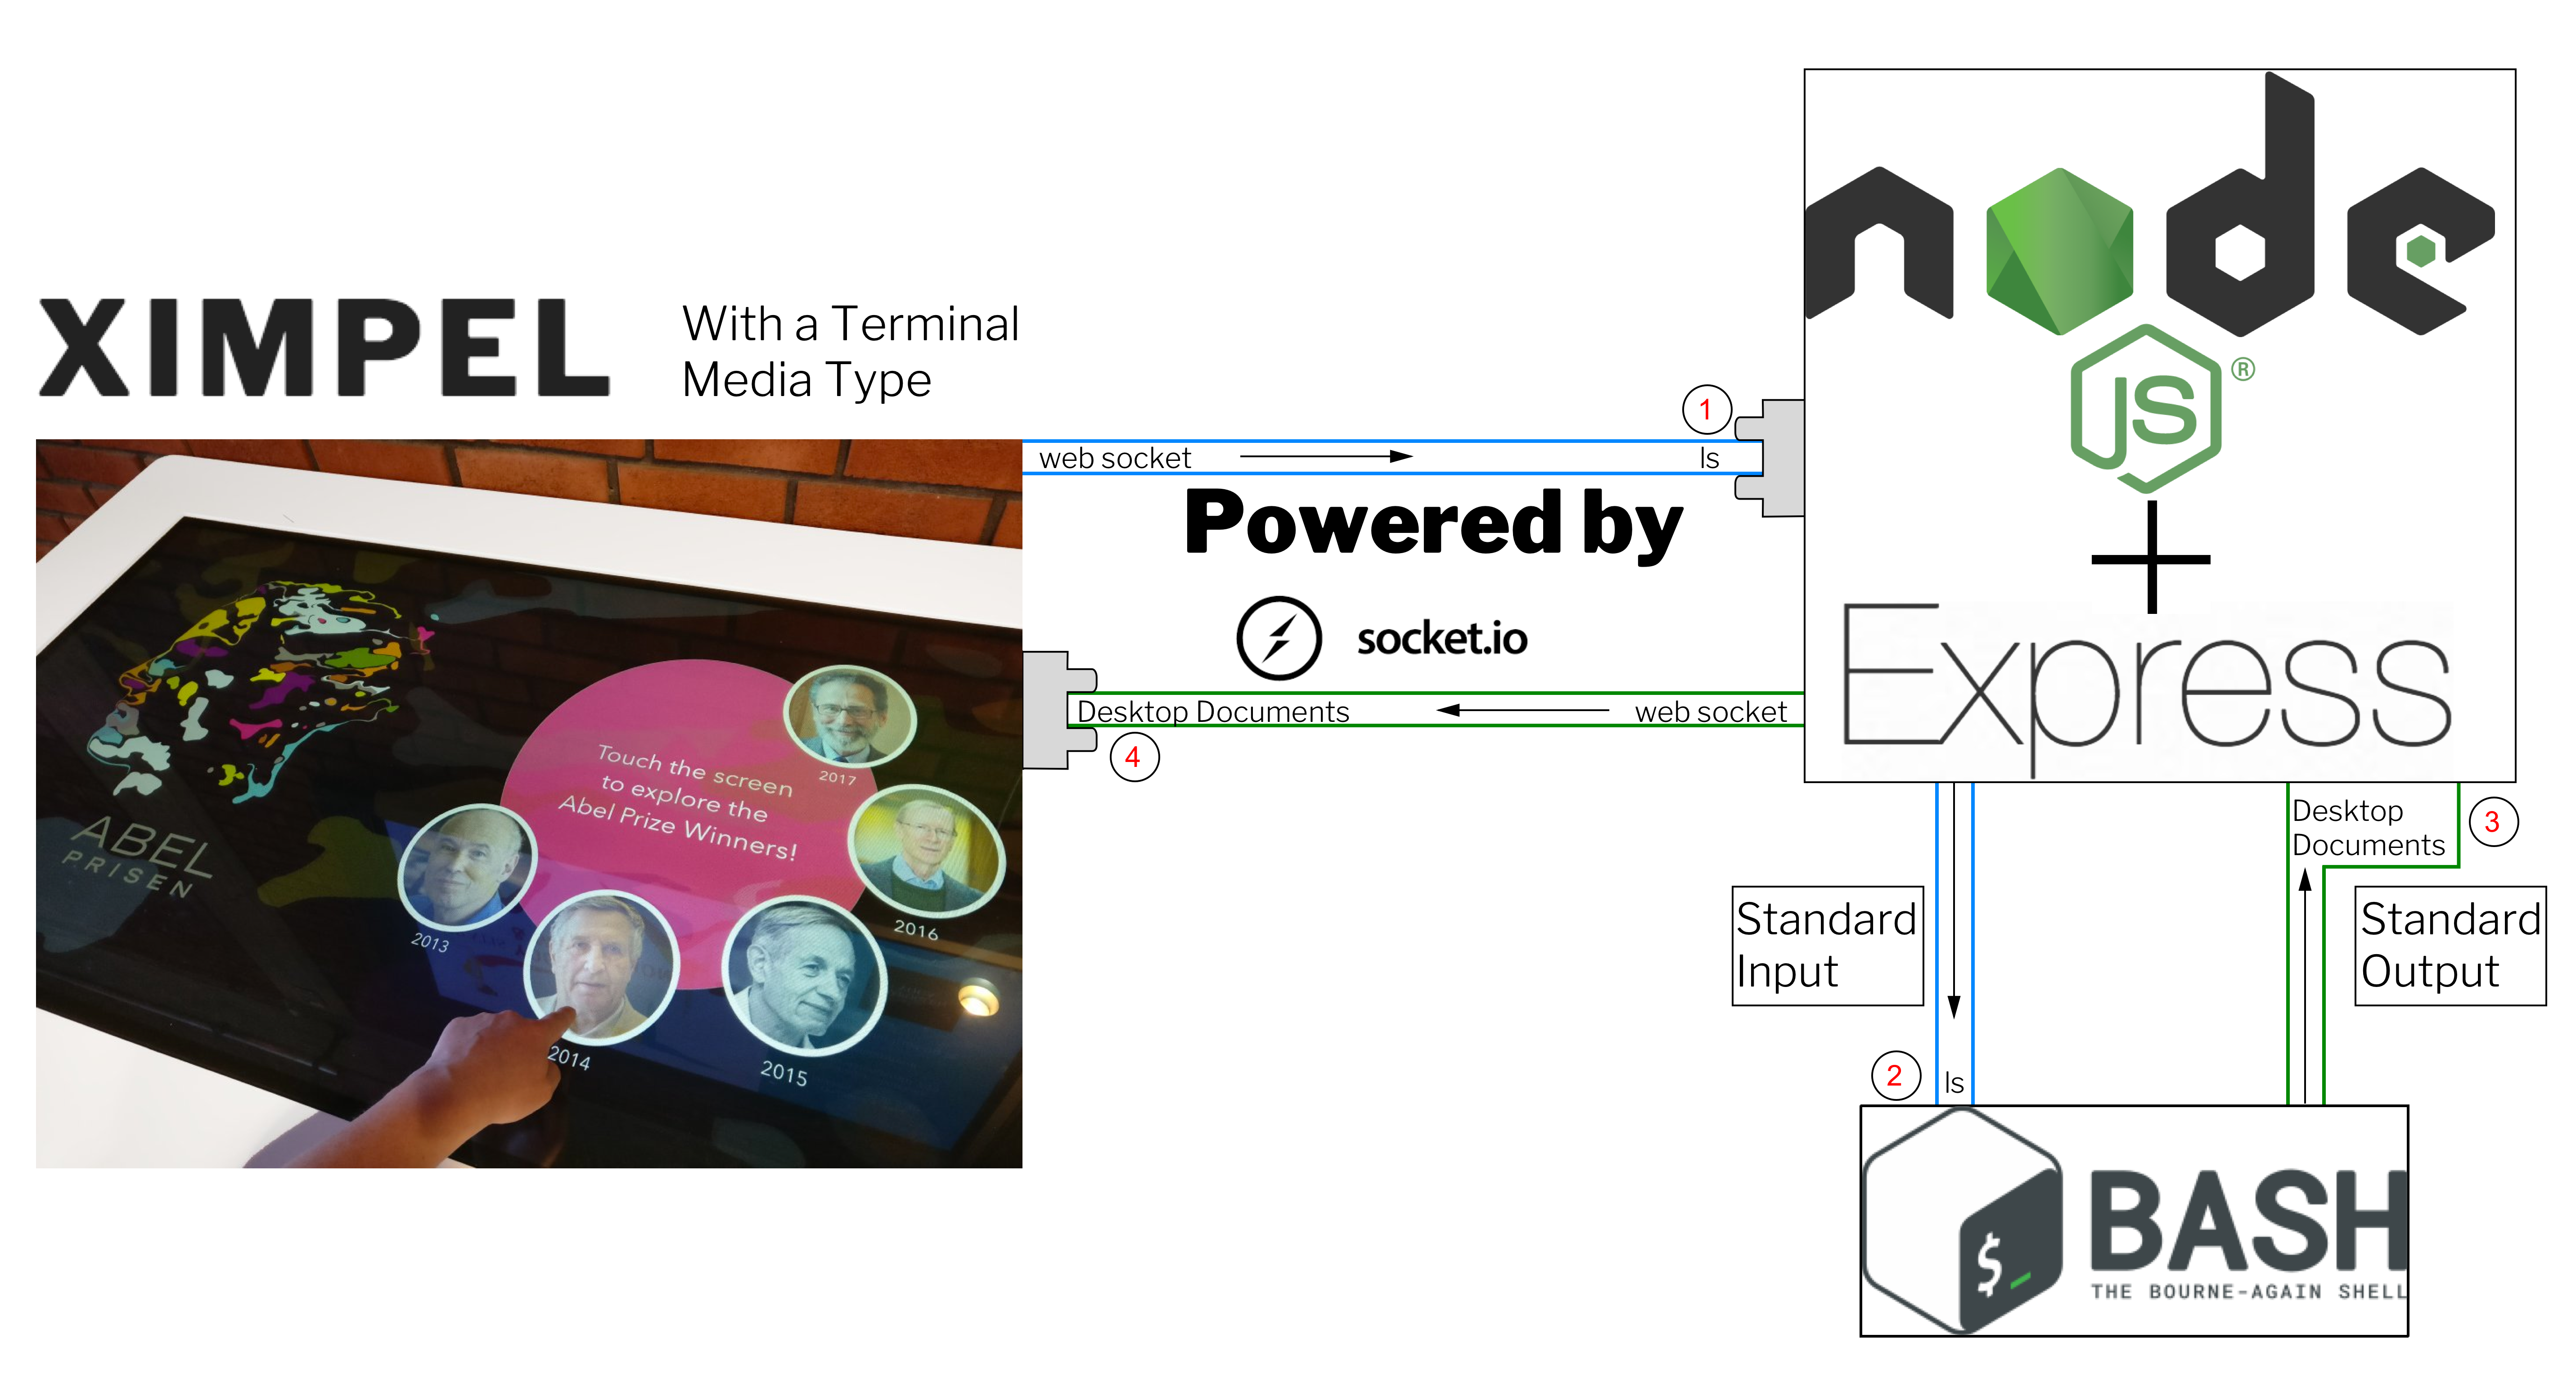
\includegraphics[width=1.35\textwidth, center]{images/terminal_architecture.png} % quotation marks make sure file name does not display
\caption{Communication example of the terminal media type. (1) The client sends a command, for example `ls`. (2) The NodeJS server sends this to a bash shell. (3) The bash shell sends a response to NodeJS, for example \textit{Desktop Documents} and (4) NodeJS sends that back to the client.}
\label{images:terminal_architecture}
\end{figure}

To conclude this section, creating a command-line tutorial has a couple of implications for XIMPEL. First, a lot of server-side web technology needs to be added such as NodeJS, ExpressJS and websockets. Furthermore, the devops tool Docker also needs to be understood. These web technologies are relatively new and not understood by all web developers and also not all web developers of XIMPEL which makes it harder to maintain XIMPEL. Second, it seems that XIMPEL is really suited for a micro service architecture. The reason for this is mostly because some media types require a server. To have a monolithic server for all possible media types in existence would harm the extensibility of XIMPEL, with microservices this danger is mitigated. Third, it is the question whether creating it as a media type is the way to go. XIMPEL also supports iframes, which means it could also have been implemented as an iframe for more control over the terminal. 

Finally to bring it back to education: XIMPEL its strength is in presenting non-linear paths, which could also be done for command-line tutorials. A serious student could perform its own manual dynamic difficulty adjustment by clicking the overlays which present possible harder or easier command-line challenges. The non-linearity of hypermedia is so built into the framework of XIMPEL that the idea is always a no brainer when one works with the framework. Yet, the idea of non-linearity is not seen in other popular online educational websites which means that hypermedia frameworks have an advantage in that aspect. 

\section{When is something hypermedia and when is it not?}
Hypermedia frameworks claim to be frameworks for rendering media items to the screen. While this is true, in the case of SMIL and XIMPEL they do much more. This is confusing, because two questions arise from this: (1) what is hypermedia? (2) Are SMIL or XIMPEL hypermedia framework or not? With regards to XIMPEL the answer is a clear no, since it is inspired by them but it is not one itself. SMIL 3.0 on the other hand is capable of interacting with parts of a web application and partially also created parts of a web application (see \cite{SMIL_lecture} around minute 25, it is a video). If all hypermedia frameworks are doing more than just enabling hypermedia content, then it needs to be established what hypermedia is and what it is not. Being able to make a distinction in that provides better vocabulary which aids categorical comparative analysis, much in the same way that the distinction between gender or sex provides categorical comparative analysis (e.g. females compared to males, two categories being compared). It may also shed light on the usefulness of non-hypermedia elements in hypermedia frameworks.

To begin answering the question: in order to answer when something is hypermedia and when something is not, it must first be asked what it means for something to be media on a computer. A literature search has been done, but unfortunately no relevant literature has been found. It is quite strange to not find literature on a very basic question such as: ``what is media?'' or its more slightly complicated version ``what is hypermedia?''

% Social media is defined as "(a) the information infrastructure and tools used to produce and distribute content that has individual value but reflects shared values; (b). the content that takes the digital form of personal messages, news, ideas, that becomes cultural products; and (c) the people, organizations, and industries that produce and consume both the tools and the content" (Howard & Parks, 2012, p. 359). Specific examples of social media sites include Facebook, Twitter and Instagram. The easy connective nature of social media sites greatly facilitates social networks, to the extent that they form a key part of this networked structure.  


The characterization of media falls into three distinct ideas, as I have seen so far: (1) mass media, (2) computer (multi)media and (3) social media. Common examples for each three is common knowledge for most people. For example, television, radio and the newspaper are seen as forms of mass media. Video, audio, images and text are seen as fundamental forms of computer media. Coincidentally the two have a very strong mapping with each other. For example, text and images appear in a newspaper. 

With social media the notion of what media is becomes more vague. Social media can be characterized as platforms where people are social on the internet. The usual suspects are: Facebook, Twitter and Instagram. But public internet forums, newsgroups or a guestbook could also be seen as social media. In all of these cases it is possible for people to communicate with each other through the use of computer (multi)media such as: video, audio, images and text (including emojis). 
Interactivity is new here and that is because with the two more old-fashioned forms of media, it always was a one way communication. 

Up until this point it could be argued that computation and manipulation of digital objects -- other than writing -- text do not need to be considered media. However, people call games media as well. And in games, everything is possible!

For our purposes, however, the characterization of media will not contain computation. A spreadsheet application is not a form of media and neither is a calculator. Other not media examples are: Finder, my text-editor, the command-line, a web browser, TeamViewer, Evernote, my FTP program, my mindmap editor, my colormeter, my screencast recording software, my vector graphics manipulation tool, Unity3D, Java, Preview, a Git viewer, Activity Monitor, my time tracker and paintbrush. This is more than eighty percent of my visible applications in my Mac OSX dock. Two applications could be considered social media, which are Colloquy (an IRC client) and Slack. However, since the information is not public (like guestbooks and forums) they may also not been seen as social media.

Finally, what all forms of media have in common is that they use the senses. For example, one hears twigs cracking slightly, above the soft noise of a fuzzing wind; furry hairs and two humongous toes are seen in the corner of an eye; a huge arm grabs your puny wrist in comparison and in a shock you realize: ``It is Bigfoot!\footnote{As much as I love furry huggable creatures I do not believe in most of them other than teddy bears for sale at the toy store.}'' If this would be a real experience, then it would not be (multi)media. However, if this experience is fabricated through: screens, paper and other various forms of technology then it is (multi)media. The multimedia researcher Anton Eli\"ens agrees with this idea. He says that multimedia is everything that uses (sensoric) media experiences such as vision and sound \cite{eliens2017:private}.

% Should I characterize media? -- leave it up to the reviewers

So what is hypermedia? Every form of media that uses vision and sound and does not contain a form of computation other than the computations that are relevant for displaying the media itself. Furthermore, hypermedia is linkable, just like hypertext. 

This means that by creating a command-line tutorial in XIMPEL, the framework has expanded beyond hypermedia. It already has been expanded beyond hypermedia in recent editions by having iframe support, so the idea that XIMPEL is only an hypermedia framework is not the case anymore.

XIMPEL is, however, mostly a hypermedia framework in its philosophy, since no programming knowledge is needed in order to create hypermedia presentations. For advanced XIMPEL users, it is more than only hypermedia. It is possibly anything that a web application could be. But XIMPEL does treat its extensions as media, even if it is an application like a command-line. This means that every extension (application or media) is able to: play, pause, stop and resume. Since it is arguable that XIMPEL is not a hypermedia framework the play, pause, stop and resume feature has less of a justification as well.

%Eliens noemt het interactive video
The conclusion for this part of the exploration is an unusual one. It is strange to wrap web applications like a terminal into custom media types. It does not seem useful to add multimedia features to this (i.e. play, stop and pause functionality). While it is possible and it works relatively well, the play, pause and stop functionality seems redundant. From a development point of view, it needs to be considered to what extent stop, play and resume functionalities should be obligatory for media types. On the other hand, a fairly easy solution is to leave an empty function body for the resume functionality. In exploration 6, I show how to program media types for mitigation of immediately stopping playback after a subject switch. So the resume and stop functionalities can be completely mitigated.

% I have to think about this conclusion

A second conclusion is that the power of XIMPEL is its playlist. For example, just by typing `<terminal>` one is able to create a complete terminal experience! This idea sparked exploration 3: recreating XIMPEL with ReactJS of which the rationale will be discussed in its relevant chapter (chapter \ref{chap:exploration3}). One of the ideas in ReactJS is similar compared to the XIMPEL playlist, which is: everything is a component. Everything in the XIMPEL playlist is a component as well.

% To do: see if you can implement this
% My final opinion on the latter question is: no not per se. XIMPEL borrows ideas from hypermedia to make sure that creating educational immersive gameplay (with media) happens a lot quicker. However, the moment XIMPEL needs to be adapted to MOOCs, the idea of XIMPEL being only a hypermedia framework should be abandoned.


% Closing paragraph
In closing, the distinction of when something is hypermedia or not justifies and delineates the relevance of hypermedia frameworks. Hypermedia frameworks keep themselves relevant by having extensibility with application components or interactibility with application parts of any platform it resides on. Furthermore, hypermedia frameworks with extensibility in mind seem not to trade any performance penalty compared to pure hypermedia frameworks, other than losing development and design focus on hypermedia features. However, a more not well-known trade-off is that by doing this a hypermedia framework becomes more complex and one could study whether it is not pedagogical to keep hypermedia frameworks simplistic, or fork hypermedia frameworks to keep the forked version simplistic. In this section it has been found that sticking too much to the hypermedia ideal harms extensibility and promotes a pure hypermedia approach. An unexpected conclusion is that the power of XIMPEL is in its playlist. Hence exploring this question led to the exploration of a software engineering question described in chapter \ref{chap:exploration3}.

\subsection{Conclusion}
How would XIMPEL need to be extended in order to create a command-line tutorial? A server-side architecture needed to be researched, implemented and a parallel player needed to be created (see chapter \ref{chap:exploration2}). This changes XIMPEL from being a front-end framework built with hypermedia philosophy to being a full-stack framework built with a hypermedia philosophy. One other way is to implement a terminal media type and not changing the nature of XIMPEL from being front-end only to full-stack would be by simulating the x86 architecture via JavaScript. This has been done before but for the constraints of the exploration described in this chapter it would take too much time.

What are the implications of mixing a hypermedia application with another application? It leads to the realization that a pure hypermedia approach has more disadvantages than advantages. This furthermore means that research should be done into the interplay of hypermedia and non-hypermedia elements in a hypermedia framework. Many hypermedia or hypermedia-like frameworks are use-case driven. An exhaustive literature review of comparing hypermedia frameworks and its use cases will shed light on a possible more abstract or generic classification of topics for which hypermedia frameworks are useful for.